\documentclass[12pt]{article}

\usepackage{amssymb}
\usepackage{bbm}
\setcounter{tocdepth}{4}
\usepackage{graphicx}
\usepackage{amsmath}
\usepackage{amssymb}
\usepackage{float}
\usepackage{array}
\usepackage{tikz}
\usepackage{morefloats}
\usepackage{pgf}
\usetikzlibrary{arrows,automata}
\usepackage{subfig}
%\usepackage[font=small]{caption}
%\usepackage{wrapfig}
\usepackage{relsize}
%\usepackage{algorithm} 
\usepackage{pdfpages}
\usepackage{algpseudocode}
\usepackage{xcolor}
\usepackage{epstopdf}
\usepackage{rotating}

\newcommand{\bx}{\mathbf{x}}
\newcommand{\by}{\mathbf{y}}
\newcommand{\bX}{\mathbf{X}}   
\newcommand{\bY}{\mathbf{Y}}
\newcommand{\bD}{\mathbf{D}}
\newcommand{\bB}{\mathbf{B}}
\newcommand{\bS}{\mathbf{S}}
\newcommand{\bb}{\mathbf{b}}
\newcommand{\bC}{\mathbf{C}}
\newcommand{\bA}{\mathbf{A}}
\newcommand{\bI}{\mathbf{I}}
\newcommand{\bc}{\mathbf{c}}
\newcommand{\bd}{\mathbf{d}}
\newcommand{\ba}{\mathbf{a}}
\newcommand{\be}{\mathbf{e}}
\newcommand{\bE}{\mathbf{E}}
\newcommand{\bSigma}{\mathbf{\Sigma}}
\newcommand{\reals}{\mathbb{\mathbf{R}}}
\newcommand{\sym}{\mathbb{\mathbf{S}}}
\newcommand{\dict}{\mathbf{\mathcal{B}}}
\newcommand{\normal}{\mathbb{\mathbf{N}}}
\newcommand{\trace}{\text{tr}}
\newcommand{\bigsum}{\mathlarger{\mathlarger{‎‎\sum}}}

\renewcommand{\algorithmicrequire}{\textbf{Input:}}
\renewcommand{\algorithmicensure}{\textbf{Initialize:}}

\begin{document}

\title{SCPLearn: Software Manual}
\author{Harini Eavani \\ Harini.Eavani@uphs.upenn.edu \\ cbica-software@uphs.upenn.edu}
\maketitle

\section{Introduction}
This software is used to calculate Sparse Connectivity Patterns (SCPs) from resting state fMRI data. SCPs consist of those regions whose connectivity co-varies across subjects. This algorithm was developed as a complementary approach to existing network identification methods. SCPLearn has the following advantages:
\begin{enumerate}
\item Does not require thresholding of correlation matrices
\item Allows for both positive and negative correlations
\item Does not constrain the SCPs to have spatial/temporal orthogonality/independence
\item Provides group-common SCPs and subject-specific measures of average correlation within each SCP
\end{enumerate}

\section{Method}
 The objective of our method is to find SCPs consisting of functionally synchronous regions, and are smaller than the whole-brain network. The information content within any one of these SCPs is also relatively low, since all the nodes within an SCP are correlated, and express the same information. Hence, if a correlation matrix were constructed for each of these SCPs, it would show two properties - (1) large number of edges with zero weights, or sparsity and (2) low information content - or rank deficiency. 

The input to our method is size $P \times P$ correlation matrices $\bSigma_n \succeq 0 $, one for each subject $n$, $n = 1, 2, \ldots, N$. We would like to find SCPs common to all the subjects, such that a non-negative combination of these SCPs generates the full-correlation matrix  $\bSigma_n$, for each subject $n$. Each of these $K$ SCPs can be represented by a vector of node-weights $\bb_k$, where $ -1 \preceq \bb_k \preceq 1$, $\bb_k \in \reals^P$. Each vector $\bb_k$ reflects the membership of the nodes to the sub-network $k$.  If $\left|\bb_k (i) \right| > 0 $, node $i$ belongs to the sub-network $k$, and if $\bb_k (i) = 0 $ it does not. If two nodes in $\bb_k$ have the same sign, then they are positively correlated and opposing sign reflects anti-correlation. Thus, the rank-one matrix $\bb_k \bb_k^T$ reflects the correlation behavior of SCP $k$. In addition, we constrain these SCPs to be much smaller than the whole-brain network by restricting the $l_1$-norm of $\bb_k$ to not exceed a constant value $\lambda$. 	

We would like to approximate each matrix $\left\lbrace \bSigma_n \right\rbrace_{n=1}^{N}$ by a non-negative combination of SCPs $\bB = [\bb_1, \bb_2, \ldots, \bb_K]$. Thus, we want
\begin{align}\label{eq:dictionary}
	\bSigma_n  &\approx  \sum_{k=1}^{K} c_n(k) \bb_k \bb_k^T + \text{diag}(\be_n)  = \bB \; \text{diag}(\bc_n) \; \bB^T  + \text{diag}(\be_n) \triangleq \hat{\bSigma_n} \nonumber   \\
    & \left| \left| \bb_k \right| \right|_1 \leq \lambda  , \quad -1 \leq \bb_k(i) \leq 1 , \quad \bc_n \geq 0, \quad \be_n \geq 0   
\end{align}
where $\text{diag}(\bc_n)$ denotes a diagonal matrix with values $\bc_n \in \reals^K_{+}$ along the diagonal. The diagonal matrix $\text{diag}(\be_n)$ is added to each approximation to make it full-rank. Thus, each subject $n$ is associated with a vector of $K$ subject-specific measures $\bc_n$ which are non-negative and reflect the relative contribution of each SCP to the whole-brain functional network in the $n$-th subject. 

We quantify the approximation between $\bSigma_n$ and $\hat{\bSigma_n}$ using the frobenius norm. Note that there is an ambiguity in amplitude between the two factors - if $\bb_k$ and $c_n(k)$ is a solution, $\alpha \bb_k$ and $c_n(k)/\alpha^2$ is also a solution for any positive scalar $\alpha$. To prevent this, we fix the maximum value in each SCP to unity; i.e., $\max_i \left| \bb_k(i) \right| =  1$. 

Bringing the objective and the constraints together, we have the following optimization problem w.r.t the unknowns $\bB$, $\bC = \left[ \bc_1, \bc_2, \ldots, \bc_n \right]$ and $\bE = \left[ \be_1, \be_2, \ldots, \be_n \right]$:
\begin{equation}
\label{eq:optProb}
	\begin{aligned}
	\underset{\bB,\bC }{\text{minimize}}
	& \; \sum_{n=1}^{N} \left| \left| \bSigma_n - \hat{\bSigma_n} \right| \right|_{F} ^{2} \\
   \text{subject to} \\
	& \quad \left| \left| \bb_k \right| \right|_1 \leq \lambda, \quad k = 1, \ldots, K,\\
	& -1 \leq \bb_k(i) \leq 1 , \quad \max_i \left| \bb_k(i) \right|  =  1,  \quad i = 1, \ldots, P\\
	&  \qquad \bc_n \geq 0 , \quad \qquad n = 1, \ldots, N \\
	\end{aligned}
\end{equation}

The objective function in the proposed model is non-convex w.r.t both unknown variables $\bB$, $\bC$ and $\bE$.  We use the method of alternating minimization to solve for the three unknowns.  At each iteration a local minimum is obtained using projected gradient descent. Such a procedure converges to a local minimum. The variable $\bB$ is initialized using k-means run on the time-points; $\bC$ and $\bE$ are initialized to randomly chosen values.

\underline{Hierarchical Framework}
This method can be applied to the data in a hierarchical fashion; first, ``primary SCPs'' are computed by running the software on the correlation matrices $\bSigma_n$. Then, for each primary SCP, multiple smaller ``secondary SCPs'' can be found by re-applying the method only for those regions that belong to the primary SCP. 

\underline{Sample weights}
This software also allows subject-specific weights as input - e.g., in cases when subjects have different numbers of time-points. In this case, the optimization objective is modified to be  $\sum_{n=1}^{N} \alpha_n \left| \left| \bSigma_n - \hat{\bSigma_n} \right| \right|_{F} ^{2}$, where $\alpha_n$ is the subject-specific weight.

\section{Software}

\subsection{Within main directory}
\begin{enumerate}
\item Detailed documentation is contained in the latex file {\color{brown}UserManual.tex} and the pdf {\color{brown}UserManual.pdf}  produced from it.
\item Author information is in {\color{brown}AUTHORS.txt}
\item All information needed to get started with the software is in {\color{brown}README.md}
\item The file {\color{brown}m2cpp.pl} is a helper perl script for doxygen. It is needed to pick up comments from MATLAB script files.
\item The file {\color{brown}INSTALL.txt} has installation and usage information.
\item {\color{brown}Doxyfile} is the configuration file for generating doxygen documentation.
\item {\color{brown}ignore.txt} contains a list of files that doxygen ignores from parsing.
\item The folder {\color{brown}docs/} will contain all the documentation once doxygen is run using {\color{brown}Doxyfile}.
\item The folder {\color{brown}src/} contains source code for SCPLearn.
\item The folder {\color{brown}licenses/} contains license information related to this software.
\end{enumerate}

\subsection{Within \texttt{src/} directory}
This software is implemeted primarily in MATLAB. For command-line argument parsing, and nifti I/O operations, python code is used.

For ease of use, the software takes as input either rsfMRI voxel time-series data in NIFTI format, or ROI time-series data in mat format. The list of nifti files is provided as a text file. 

It also takes as input the node definitions as an atlas in NIFTI space. This atlas must have the ROI regions numbered $1, 2, 3, \ldots$ and must be in the same space as the subject data. 

\begin{enumerate}
\item Main function is {\color{blue}SCPLearn.py}. This function parses the input arguments and calls ``ComputeROIAverages.py''.
\item {\color{blue}ComputeROIAverages.py} reads the rsfMRI data and the node definitions. It extracts average time-series of each ROI for each subject and saves it in ``.mat'' files.
\item These mat files are loaded into MATLAB using the function {\color{magenta}SCPLearnFromMatFiles.m} . Then, based on the input parameters, either (1) {\color{magenta}SCPLearn.m} is called, which computes only primary SCPs,  or (2) {\color{magenta}SCPLearn\_two\_level.m} is called which computes both primary and secondary level SCPs.
\item Both the above functions call {\color{magenta}BlockSolverLowRankFrob.m}, which implements the alternate minimization strategy discussed in the previous section. This function calls (1) {\color{magenta}BSolver\_lowrank\_frob.m} (2)  {\color{magenta}CSolver\_lowrank\_frob.m}  (3)  {\color{magenta}ESolver\_lowrank\_frob.m} until termination criteria are met.
\item {\color{magenta}BSolver\_lowrank\_frob.m} calls two functions (1) {\color{magenta}spg\_04262015.m} which implements projected gradient descent. (2) {\color{magenta}ProjectionOnUnitBoxSimplex.m} implements the projection function for the sparse basis.
\item After the MATLAB code has finished running, {\color{blue}SCPLearn.py} calls {\color{blue}replaceLabels\_nib.py}. This python code replaces the labels in the atlas with the values of the nodes in each SCP. In this manner, for each SCP, a nifti image is written to disk.
\item The set of python functions in {\color{blue}SCPUtils.py} are used for error checking, handling exceptions, file check, etc
\item The MATLAB functions {\color{magenta}SCPLearn\_SplitSample.m}, {\color{magenta}CompareSCPs.m},{\color{magenta}Hungarian.m} implement split-sample SCP reproducibility and error calculation, as described and used in the main paper.
\item The python script {\color{blue}makeAll.py} calls mcc to build {\color{magenta}SCPLearnFromMatFiles.m} as an mcc-executible. It then copies all python files to the install directory.
\end{enumerate}

\section{Installation}
\subsection{Dependencies}
This software has been primarily implemented for Linux operating systems.
\begin{itemize}
\item MATLAB Compiler mcc version 5.2 (R2014B)
\item MATLAB R2014B
\item Python 2.7.9
\item Python library numpy 1.7.2
\item Python library scipy 0.15.1
\item Python library pandas 0.16.2
\item Python library nibabel 2.0.1
\end{itemize}
Make sure all dependencies are met before proceeding with install.

\subsection{Generating standalone executables}

\begin{enumerate}
\item Within the \texttt{src/}  directory, run \texttt{makeAll.py}  with the location of the install directory as the argument:

\texttt{makeAll.py <installDir>}

\item Add the install directory to your path by running the following command. 

Replace \texttt{\${installDir}} with the location of the install directory from step 1 above.

\texttt{ export PATH=\${PATH}:\${installDir} }

\end{enumerate}


\subsection{Generating documentation}


Run \texttt{doxygen Doxyfile} from the parent directory.
The documentation is built in \texttt{docs/*}. Open \texttt{ docs/index.html} in your favorite browser to begin.

\section{Usage}
\begin{verbatim}
Usage: SCPLearn.py [OPTIONS] 

Required Options:
[-d --data] Specify the text file with list of nifti files (required) 
            *** OR ***
            Specify the text file with list of mat files (required) 
            Each mat file must contain a variable named 'ts'
            'ts' must be a matrix of time-series, size = #ROIs X #timepoints
                    
[-m --mask]   Specify the nifti ROI/parcel/atlas file (required)
[-p --prefix] Specify the prefix of the output file  (required)
    
Options:
[-s --sparsity] 	Specify the sparsity constraint as positive value. 
                 Default = nROIs/8 
[-n --numberOfSCPs] 	Specify the number of SCPs as a number. 
                     Default = 10.    
[-r --pruning]  Specify the pruning threshold as a value between [0,1]. 
                Default = 0.7.    
[-l --levels]  	Hierarchical learning of SCPs. Not run by default. 

[-o --outputDir] The output directory to write the results. 
                 Defaults to the location of the input file
[-w --workingDir] Specify a working directory. 
                  By default a tmp dir is created and used
[-u --usage | -h --help] Display this message
[-v --verbose]           Verbose output
[-V --Version]           Display version information

Example:
SCPLearn.py -d list_of_nifti_files.txt -m Grasp_level5.nii -p SCP_results \
                    -n 10 -o /sbia/sbiaprj/BLSA -v
    
Example list_of_nifti_files.txt without sample weights:
ProjName_subj_165464.nii.gz
ProjName_subj_26464.nii.gz
ProjName_subj_1054.nii.gz......

Example list_of_nifti_files.txt with sample weights:
ProjName_subj_165464.nii.gz,172
ProjName_subj_26464.nii.gz,160
ProjName_subj_1054.nii.gz,120......      
\end{verbatim}
To run this software you will need:
\begin{enumerate}
\item Text file with list of NIFTI files
\item NIFTI file with node definitions
\end{enumerate}
In the output directory, the software returns:
\begin{enumerate}
\item One NIFTI file for each SCP that is generated, with file name \texttt{$<$prefix$>$\_SCP\_\#.nii.gz}
\item A \texttt{$<$prefix$>$\_SCP\_Coeffs.csv} file with the SCP coefficients for all the subjects, indexed by the NIFTI filename that was input
\item A \texttt{$<$prefix$>$\_SCP\_basis.csv} file with the SCP basis, in csv format
\item A \texttt{$<$prefix$>$\_SCPs.mat} file with all the outputs in MATLAB ``.mat'' format
\item A \texttt{$<$prefix$>$\_ts.mat} file with the average time-series from all the subjects in MATLAB ``.mat'' format
\item A \texttt{$<$subject$>$\_$<$atlas$>$.mat} file with the average time-series for each subject 
\end{enumerate}


\section{Testing}
To test the software, we have provided synthetic nifti as well as mat data for ten ``subjects''. These are located in \texttt{ src/test}. 

To run the software on the synthetic data, run the following command from the \texttt{ src/} folder :

\texttt{SCPLearn.py -d test/nifti\_list.txt -p test\_2d -m test/test\_2d\_mask.nii.gz -o test/ -n 3 -s 10}  \\

or 

\texttt{SCPLearn.py -d test/mat\_list.txt -p test\_2d -m test/test\_2d\_mask.nii.gz -o test/ -n 3 -s 10}

This command should return three SCPs, saved as nifti files in  \\
\texttt{  src/test/test\_2d\_SCP\_{1,2,3}.nii.gz } \\
along with other output. 

By design, three patterns were used as ``ground-truth'' SCPs to generate the synthetic data; a cross, a circle and a square.
Was SCPLearn able to clearly separate these three patterns in the output? You can compare your result to the results in \texttt{test/Test\_2d\_all.png}. This image is also shown in Figure \ref{fig:test}.

\begin{figure}
\centering
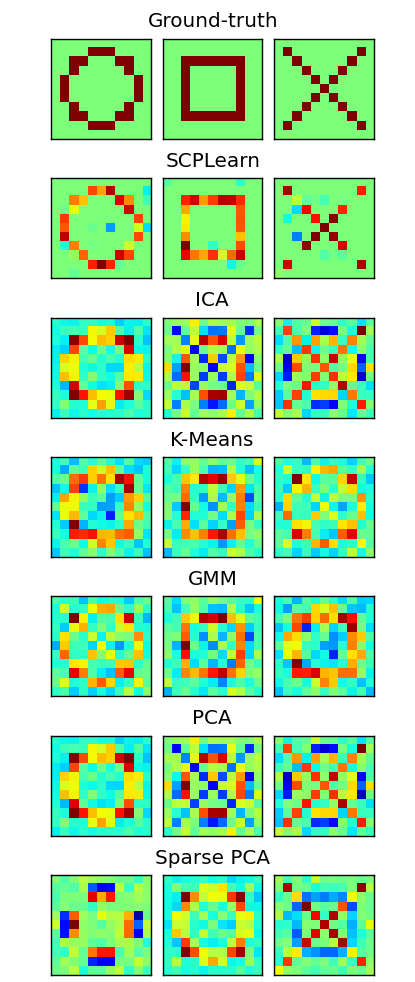
\includegraphics[scale=0.8]{src/test/Test_2d_all.png}
\caption{Synthetic SCPs used for testing. Results from SCPLearn and other approaches are also shown.}
\label{fig:test}
\end{figure}

In addition, the NetSim-based synthetic data used in the original paper is provided in \texttt{netsim\_data\_05262014\_timeseries.mat}. To test the MATLAB code using this data, run \texttt{testSCPLearnCode.m} from the MATLAB command line.

\section{Citation}
If you find this code useful, please cite: \\
\texttt{Eavani, H., Satterthwaite, T. D., Filipovych, R., Gur, R. E., Gur, R. C.,  Davatzikos, C. (2015). Identifying Sparse Connectivity Patterns in the brain using resting-state fMRI. Neuroimage, 105, 286-299.}
\end{document}

%%
%% End of file `elsarticle-template-harv.tex'.
